\section{Results}
\label{sec:results}

This section reports descriptive results derived from the repository artifacts available in the analyzed snapshot. The measures characterize direct-generation architecture CSVs, their execution traces, and the static source corpus. They do not constitute human-quality ratings or an external validity assessment.

\subsection{Result availability and artifact quality}

A read-only artifact calculation discovered 48 direct-generation run identities. Of these, 48 yielded a calculable final architecture CSV. Every included direct-generation run resolved to a calculable final architecture CSV. 4 TNTConcept metadata paths selected missing canonical filenames; each was reconciled in memory to the unique CSV in the same condition folder. The source metadata and output artifacts were not modified. All 42 audit notices were repeated metadata records; the latest successful record was selected for each logical run.

The structural parser found no malformed service rows, duplicate service names or communications, invalid communication targets, self-communications, or responsibilities shorter than the configured five-word threshold.

\begin{table}[t]
\centering
\small
\begin{tabular}{lrl}
\toprule
Artifact status & Count & Scope or treatment \\
\midrule
Discovered run identities & 48 & Current outputs/ inventory \\
Calculable final architecture CSVs & 48 & Included in architecture metrics \\
Valid direct outputs & 48 & Eight projects; included in direct aggregates \\
In-memory metadata-path recoveries & 4 & Unique sibling CSV selected; source artifacts unchanged \\
Outputs without calculable final CSV & 0 & Excluded from architecture aggregates \\
Recorded audit notices & 42 & Discovery, metadata, architecture, or trace notices retained \\
Within-condition stability pairs & 0 & One run per condition; stability Jaccard unavailable \\
\bottomrule
\end{tabular}
\caption{Availability of calculated artifacts in the analyzed repository snapshot.}
\label{tab:result-availability}
\end{table}


The direct-generation snapshot has one run per project--provider--prompt condition. Therefore, there are no within-condition run pairs from which to estimate output stability; the corresponding Jaccard stability values are unavailable rather than zero. No human-evaluation data are included in this replication package.

\subsection{Static characteristics of the source corpus}

The static analysis covers 8 Java systems. The corpus ranges from Jokul (967 effective source lines) to TNTConcept (97,785 effective source lines), providing a marked variation in codebase scale and package-level structure. Figure~\ref{fig:static-corpus-profile} visualizes the variation in effective source lines, analyzed type files, and distinct internal package dependencies. The full corpus profile is reported in Table~\ref{tab:static-corpus}.

\begin{figure*}[t]
\centering
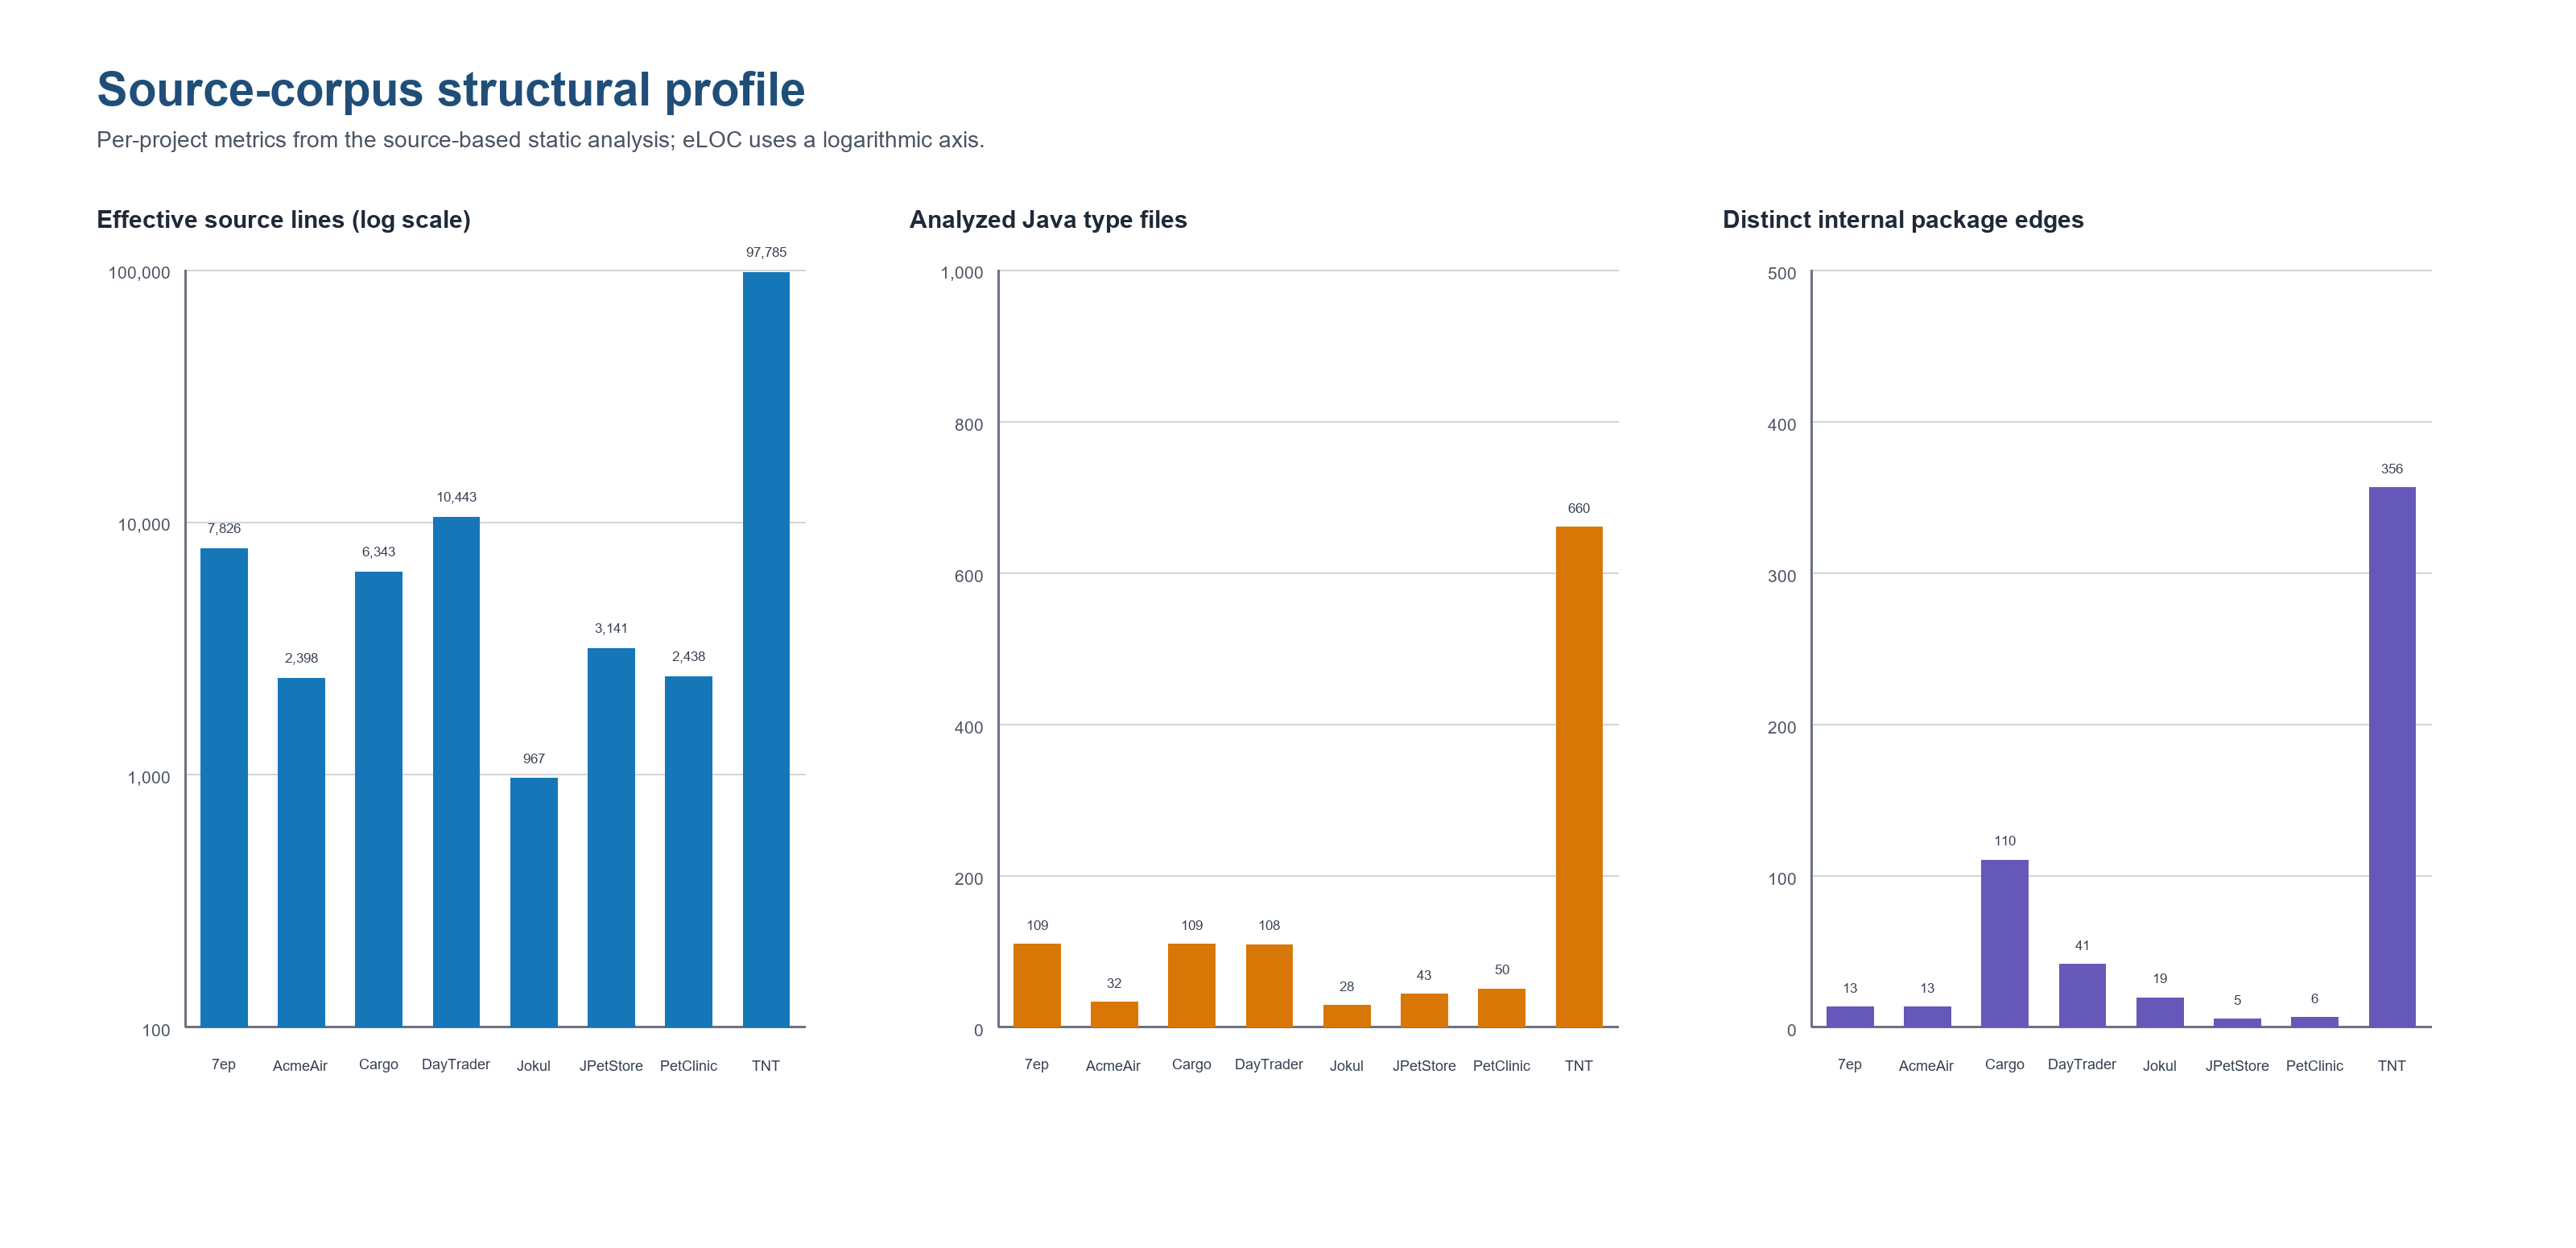
\includegraphics[width=\textwidth]{docs/article_results/figures/fig_static_corpus_profile.png}
\caption{Static source-corpus profile. Effective source lines are shown on a logarithmic scale; package edges are distinct internal import-derived relations.}
\label{fig:static-corpus-profile}
\end{figure*}

\begin{table}[t]
\centering
\small
\resizebox{\linewidth}{!}{%
\begin{tabular}{lrrrrrrrr}
\toprule
Project & Build files & Type files & Packages & Methods & eLOC & Internal imports & Internal edges & Entrypoints \\
\midrule
7ep & 3 & 109 & 14 & 670 & 7,826 & 112 & 13 & 14 \\
acmeair & 1 & 32 & 10 & 151 & 2,398 & 38 & 13 & 8 \\
cargo-tracker & 1 & 109 & 28 & 617 & 6,343 & 355 & 110 & 5 \\
daytrader7 & 4 & 108 & 11 & 1,011 & 10,443 & 235 & 41 & 45 \\
Jokul & 1 & 28 & 12 & 119 & 967 & 45 & 19 & 5 \\
jpetstore & 1 & 43 & 6 & 366 & 3,141 & 61 & 5 & 1 \\
pet-clinic & 2 & 50 & 7 & 204 & 2,438 & 34 & 6 & 10 \\
TNTConcept & 3 & 660 & 72 & 15,401 & 97,785 & 2,691 & 356 & 0 \\
\bottomrule
\end{tabular}
}
\caption{Static source-corpus profile. Type files are analyzed Java type files; internal edges are distinct import-derived package relations.}
\label{tab:static-corpus}
\end{table}


Supplementary Tables~S3--S5 report the remaining source-structure, code-volume, heuristic-classification, and import-derived dependency fields for all eight systems.

\subsection{Structural properties of direct-generation outputs}

Across the 48 valid direct-generation outputs, the median service count was 4 (IQR 3--5), and the median number of valid directed communications was 9 (IQR 6--13). Median communication density was 0.67, while the median responsibility length was 23.8 words per service. These values summarize output structure and lexical detail; they do not establish that a larger or denser architecture is better.

\begin{table}[t]
\centering
\small
\begin{tabular}{llrrrrr}
\toprule
Provider & Prompt & n & Services & Valid links & Density & Responsibility words \\
\midrule
OpenAI & zero-shot & 8 & 3.5 [3.0, 4.0] & 6.0 [6.0, 10.0] & 0.92 [0.79, 1.00] & 31.0 [27.0, 32.9] \\
OpenAI & few-shot & 8 & 3.5 [3.0, 4.2] & 6.0 [6.0, 11.5] & 0.82 [0.71, 1.00] & 25.5 [21.9, 28.9] \\
Anthropic & zero-shot & 8 & 4.5 [3.8, 5.0] & 9.5 [5.5, 11.5] & 0.60 [0.43, 0.71] & 40.3 [33.8, 42.9] \\
Anthropic & few-shot & 8 & 4.5 [3.0, 5.2] & 9.5 [4.8, 14.2] & 0.66 [0.50, 0.73] & 23.8 [23.0, 25.1] \\
DeepSeek & zero-shot & 8 & 4.5 [4.0, 6.0] & 10.5 [6.8, 13.2] & 0.53 [0.46, 0.65] & 13.6 [9.9, 17.9] \\
DeepSeek & few-shot & 8 & 4.5 [3.8, 5.2] & 9.5 [7.0, 12.2] & 0.53 [0.42, 0.67] & 13.7 [10.8, 15.6] \\
\bottomrule
\end{tabular}
\caption{Descriptive structural statistics for valid direct-generation outputs. Entries are median [Q1, Q3] across available systems.}
\label{tab:direct-by-condition}
\end{table}


\begin{figure*}[t]
\centering
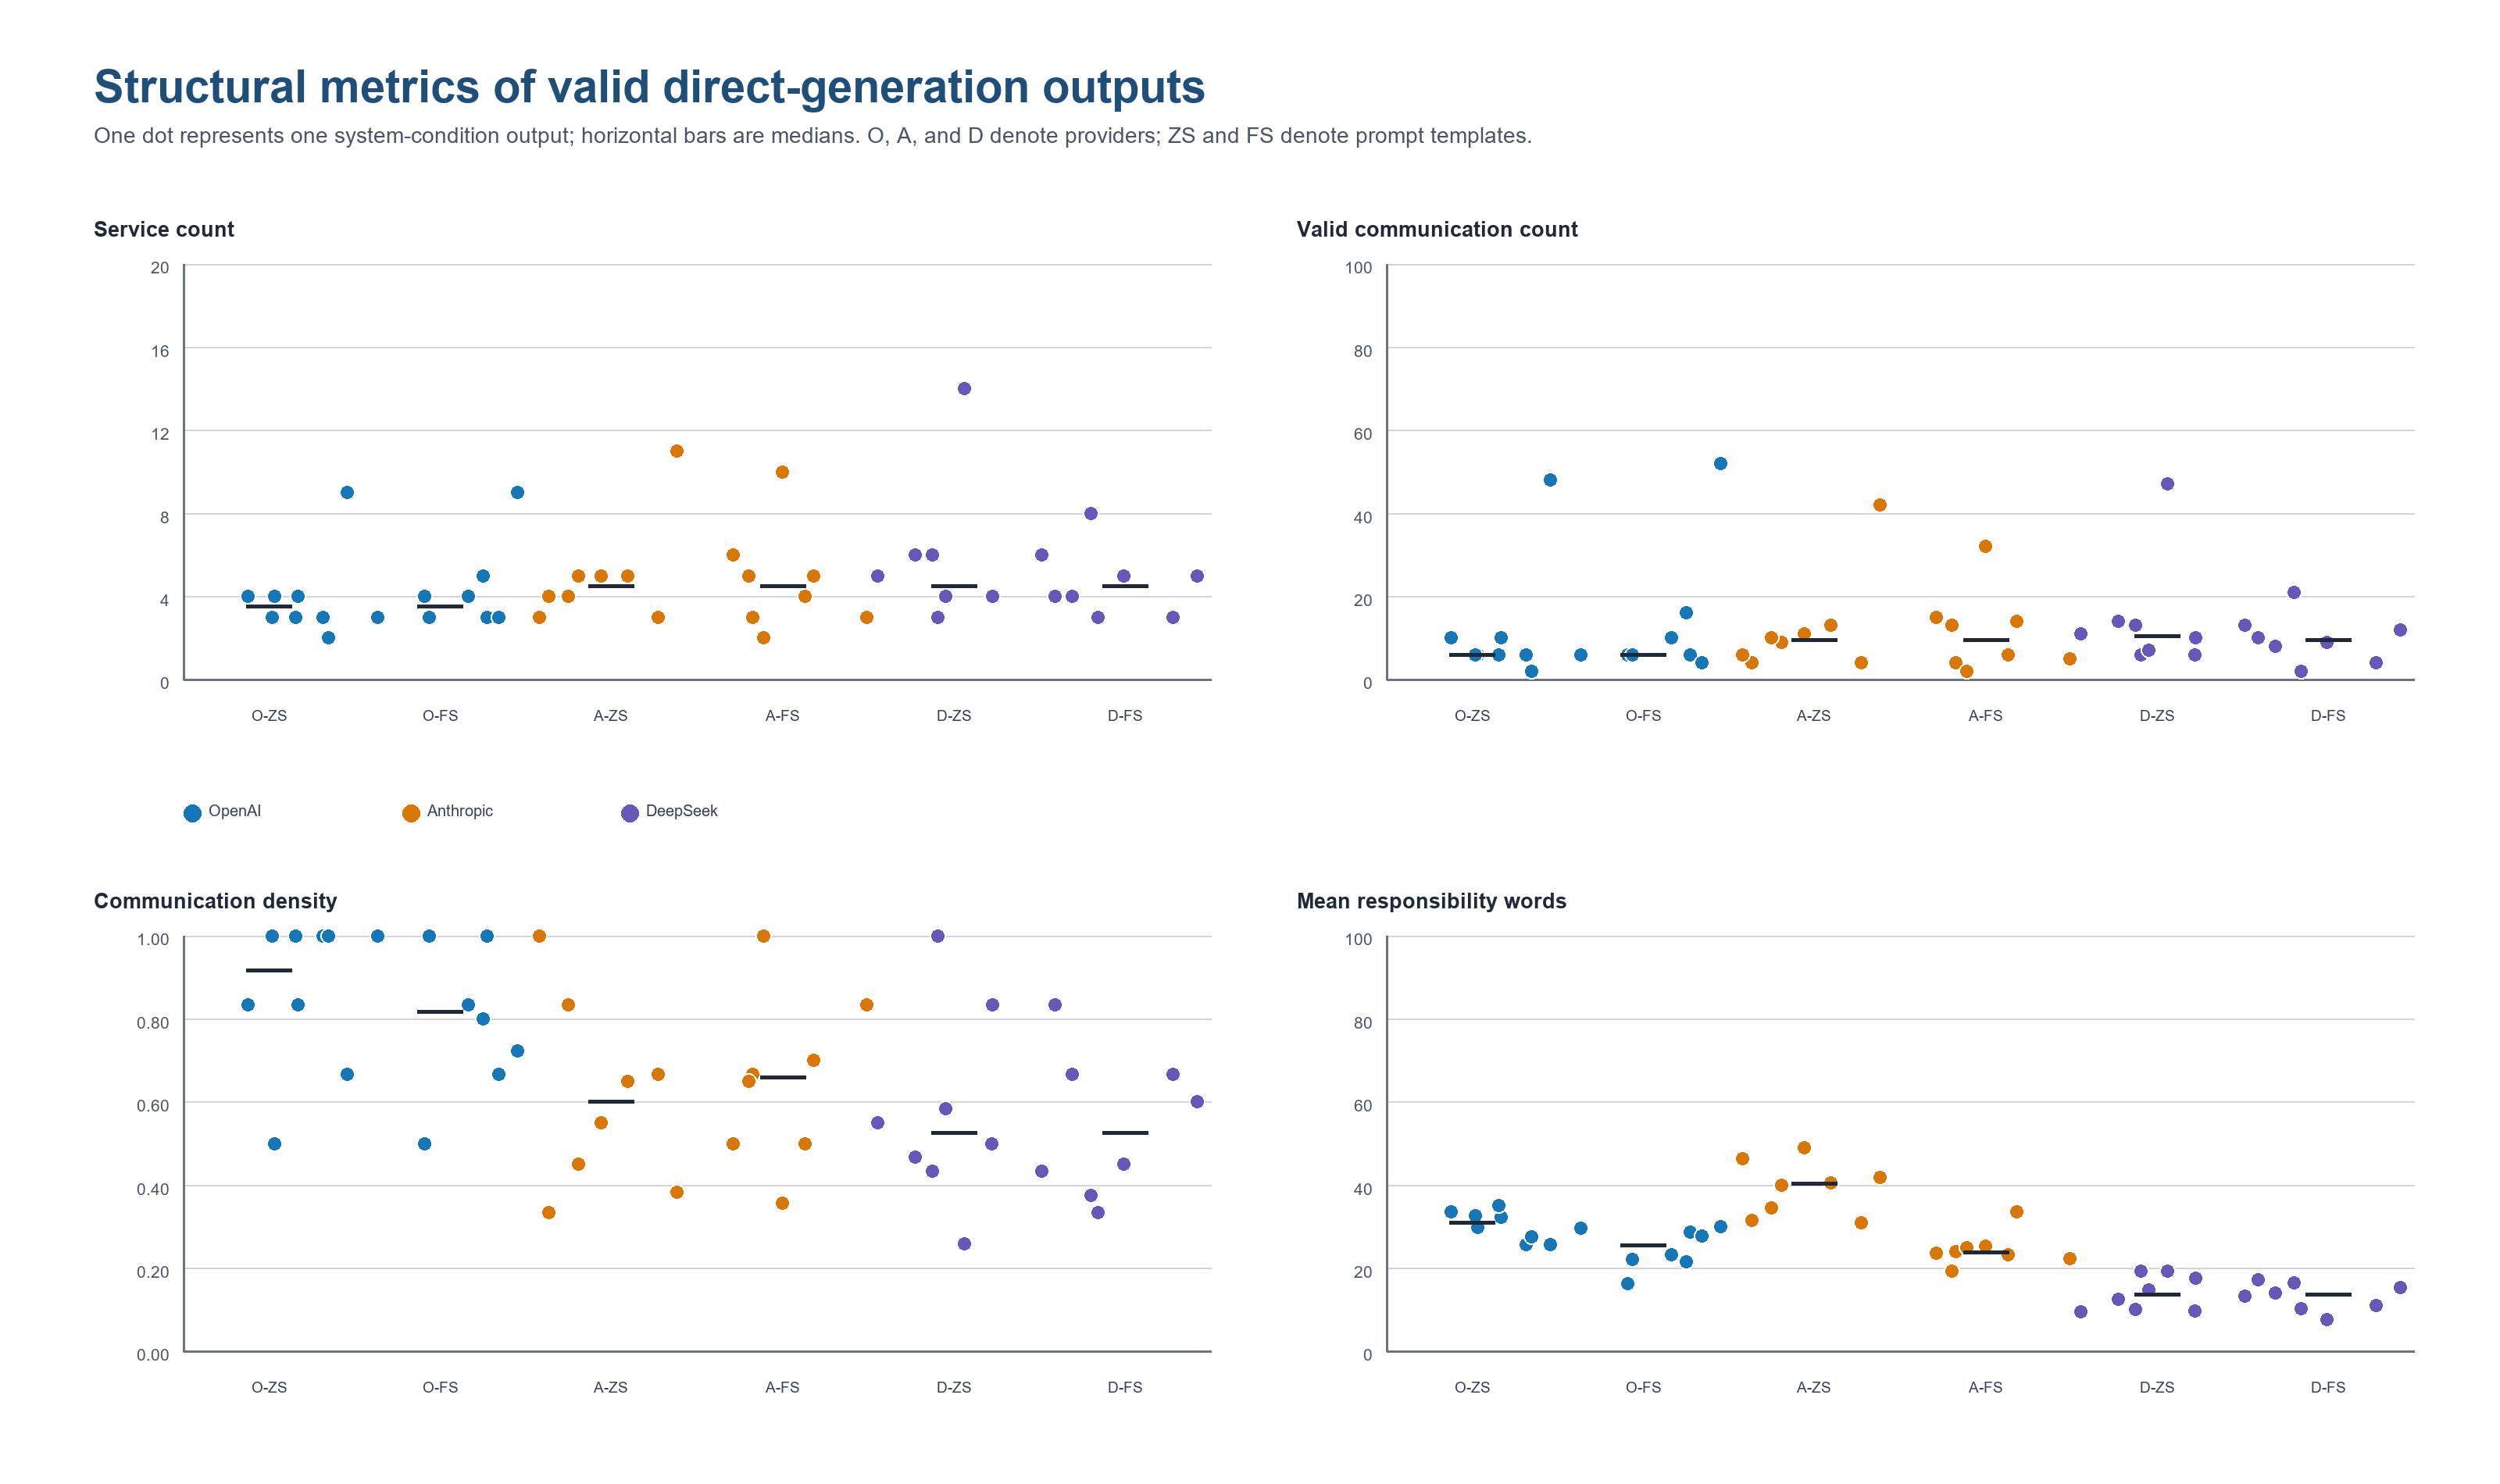
\includegraphics[width=\textwidth]{docs/article_results/figures/fig_direct_architecture_metrics.png}
\caption{Distribution of structural metrics across valid direct-generation outputs. Each point is one system-condition output, and horizontal bars denote medians within a provider--prompt condition.}
\label{fig:direct-architecture-metrics}
\end{figure*}

Supplementary Table~S1 provides the complete descriptive summary for every calculated architecture metric, while Supplementary Table~S2 provides all direct-generation trace metrics. The row-level exports accompanying this section preserve every calculated value, including malformed rows, invalid targets, isolation, reciprocity, responsibility-length, lexical-overlap, retry, duration, prompt-volume, role, and final-snapshot measures.

\subsection{Interpretation boundary}

The reported measures are deliberately descriptive. Structural regularity, prompt volume, and trace duration are useful audit signals, but none independently demonstrates requirement coverage, domain correctness, implementability, or superiority. Those claims require the planned expert-review data and, where appropriate, independent architectural validation.
